\chapter{Semantic Web Basics} \label{ch:briefintrosemanticweb}

Ontology is the philosophical study of the nature of being, existence, or reality. It concerns about ``what is everything'' and ``how to define everything'' in the context of inductive and deductive reasoning. It discusses how we as human abstract and preserve knowledge.

Ontology inspires people in computer science about how we can store and exchange information efficiently using the internet. The solution is known as the semantic web, an internet-based knowledge base schema. The internet powered by semantic web (together with other technologies) defines Web 3.0, a new-generation internet framework.

Notice that there are subtle differences between ``internet'' and ``Internet''. The lower case ``internet'' refers to the technology that bridges machines to form a network of any size, and the upper case ``Internet'' refers to the specific internet that links the entire world together. In this part of the notebook, however, they are used interchangeably.

\section{Web of Data}

The internet is a technology that enables information exchange among machines. With the power of the internet, a user can obtain the information he needs from remote servers, databases, or knowledge bases.

In the early days, the use of internet required professional skills. Nowadays, everyone can access the internet using a graphical-interface browser that he can easily find on a computer or a mobile device. Public knowledge bases such as Wikipedia has made obtaining information much easier.

\subsection{Web 1.0 and 2.0}

Under the \mync{Web 1.0} framework which was popular in the early stage of internet development, information is stored on individual servers in a static manner. A user can browse the contents, but he cannot edit them. It is essentially a one-way data transmission. The ``authority'' such as a news company provides the information, and the users consume it. Examples of Web 1.0 implementations include news websites, static web gallery, etc.

One-way data transmission in Web 1.0 cannot meet the expectation from the users who want to share their information to other users on the internet. Thanks to the advent in information science and communication, under the \mync{Web 2.0} framework users can interact with the internet bidirectionally. A user can search and filter data from the servers and even upload his own data and share it with others. The internet became far more powerful in terms of information exchange. The source of information does not necessarily come from the authority. The users are generators and consumers of information at the same time. Examples of Web 2.0 implementations include Blog, Twitter, YouTube and Weibo.

Web 2.0 is extremely popular and successful even to date. Yet, under the background of industry 4.0, big data and data-driven modeling of almost everything, there are still limitations and downsides to Web 2.0 that we would wish to improve.

One of the biggest challenges that we encounter with Web 2.0 is how to quickly locate the information we want among the vast amount of irrelevant data. Conventionally in Web 2.0, keyword-based searching engines are used. These searching engines do not comprehend the contextual knowledge of the contents, and as a result they may fail to return what a user truly expects. The user often needs to further manually pick up relevant information from the searching results. Nowadays searching engines are becoming smarter, and they can sometimes pre-filter the results. Nevertheless, it is still quite common that many returned results are useless to the user. Keyword-based engines also struggle with polysemous, synonyms and implicit information from pictures in the searching range, again due to the lack of understanding of the contents.

The problem here, however, is not caused by the searching engines alone.  It is rather that the information stored on the internet does not come with its corresponding semantics in the first place. Today most of the information on the internet is stored in HTML format. HTML tells only the contents but not the meaning behind them. It is difficult for a machine to understand the meaning of the information from HTML corpus. This potentially makes it difficult for a machine to retrieve data efficiently. Even with the recent breakthrough in LLM enabling the machine to summarize articles, it is still unpractical for it to go through all the returned contents of a searching engine which sometimes contains hundreds of pages of information.

Structure determines functions. To solve the problem once for all, new data storage and sharing model needs to be introduced.

\subsection{Web 3.0}

The goal of \mync{Web 3.0} is to allow more efficient information retrieval and sharing using the internet. Ideally, we would want the searching engine to truly understand the user's demand, and return only the most relevant information summarized in a nice manner. If there is no readily available response on the internet, the searching engine shall derive the response based on existing information, i.e., it should be capable of doing simple reasoning. 

For this purpose, there are at least the following two development trends:
\begin{itemize}
  \item Let the LLM-based AI remember all the knowledge. The LLM should be smart enough to precisely capture what the user wants and get back to him with useful and accurate information. This leads to chatbots and copilots.
  \item Create a powerful and flexible NoSQL database. Make the information in the database readable for both humans and machines, and somehow integrate the semantics of the contents into the database. This leads to \mync{semantic web}.
\end{itemize}

In practice, it is most recommended to use both LLM-based AI and semantic web simultaneously. This is because both LLM-based AI and semantic web have drawbacks when used alone.
\begin{itemize}
	\item LLM-based AI
	\begin{itemize}
		\item Time and computational load wise expensive to expand the knowledge base;
		\item Lack the ability of reasoning;
		\item A chance to produce misleading information;
		\item Cannot be merged and migrated easily because the ``knowledge'' in the form of regression coefficients is not human or machine readable;
	\end{itemize}
	\item Semantic web
	\begin{itemize}
		\item Steep learning curve to use;
		\item Not good at summarizing and formatting the response in a human-friendly manner.
	\end{itemize}
\end{itemize}

Web 3.0 schema focuses on semantic web. The word ``semantics'' in this context specifically refers to the relations of objects and properties that can be used for machine-driven descriptive reasoning. See later sections for details. Semantic web is so important that it is often considered synonymous with Web 3.0, although the broader vision of Web 3.0 includes other features as well.

Another feature of Web 3.0 is distributed storage of information. Distributed storage has both advantages and disadvantages. On one hand, it provides higher resilience against data loss. On the other hand, it adds challenges to the searching and collecting of information during the querying. Technologies like \myabb{InterPlanetary File System}{IPFS}, blockchain, and distributed databases are used to address these challenges.

This notebook discusses the technologies used in semantic web such as \mync{resource description framework}[RDF] model, \mync{RDF schema}[RDFS] and \mync{web ontology language}[OWL]. We will see how we can use semantic web to collect and organize information, and create a knowledge base for both humans, machines, and AI.

\subsection{Semantic Web Vision}

Semantic web database is ``semantic'' due to its data model. Semantic web data model not only stores objects and their properties, but also the relationships among objects and properties. The relationships, often represented by graphs, can be used for descriptive logic reasoning. The logic reasoning allows new information to be derived based on existing facts. In addition, semantic web is more scalable, reusable and reader-friendly for both humans and machines comparing with AI methods.

Many research institutes and organizations have tried building semantic webs of different scales. An example is DBPedia (\textit{dbpedia.org}). The goal of DBPedia is to create something like Wikipedia, but using semantic web.

\subsection{Semantic Web Stack} \label{subsec:semanticwebstack}

A commonly seen semantic web stack looks like Fig. \ref{fig:semanticwebstack}. 

\begin{figure}[htbp]
	\centering
	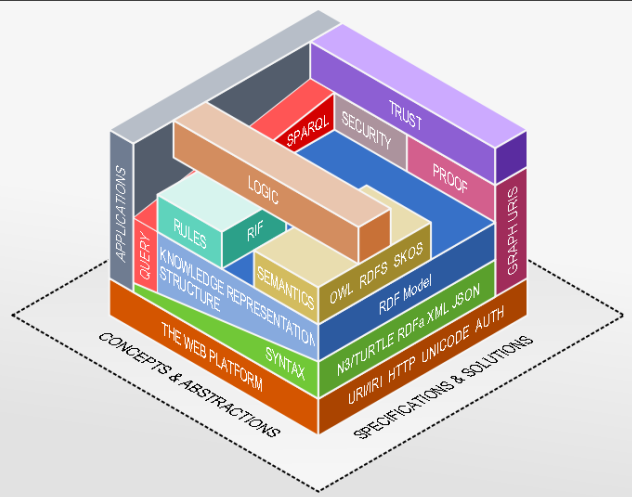
\includegraphics[width=0.8\textwidth]{chapters/part-4/figures/semanticwebstack.png}
	\caption{Semantic web stack \cite{semanticwebstack}.}
	\label{fig:semanticwebstack}
\end{figure}

The layers and components in each layer are briefly introduced as follows.
\begin{itemize}
	\item Web platform layer
	\begin{itemize}
		\item \myabb{Uniform resource identifier}{URI} and/or internationalized resource identifier, often a string used to identify and trace an information resource.
		\item Communication protocols, such as HTTP and HTTPS.
		\item Text encoding methods, such as unicode, utf-8.
		\item Authentication methods.
	\end{itemize}
	\item Syntax
	\begin{itemize}
		\item File formats to store information, such as RDF/XML and JSON-LD.
	\end{itemize}
	\item Knowledge representation, semantics, and interfacing tools
	\begin{itemize}
		\item RDF (by default) which uses triples to represent a graphical database.
		\item RDFS and OWL which expand the capability of RDF model.
		\item SPARQL which is the recommended language for semantic web query (SPARQL 1.0) and manipulation (SPARQL 1.1).
	\end{itemize}
	\item Logic
	\begin{itemize}
		\item Logic statements and reasoning that semantic web supports for query.
		\item Rules that describes what query can be executed.
	\end{itemize}
\end{itemize}

The knowledge and semantics are stored using the RDF/RDFS model. The RDF/RDFS is often further powered by OWL. RDF serves as the foundation with the basic structure. RDFS expands the capability of RDF by introducing new vocabularies such as ``class'', ``subclass'', ``property''. And finally OWL enables a set of tools to define complex ontologies and create rigorous and complex semantics. As an analogy, think of RDF as the paper and pencil, RDFS the 24-color crayon set, and OWL the painting skills. Together they make a sophisticated and richly structured picture.

It is worth mentioning that many syntax such as RDF/XML can be used as the markup languages to describe RDF/RDFS/OWL used in a semantic web. More details are introduced in later chapters.

\mync{SPARQL Protocol and RDF Query Language}[SPARQL] is the recommended query language for querying and manipulating the semantic web. It allows a user to search, retrieve, and modify information stored in the RDF model. The syntax of SPARQL is designed to look similar with SQL, and many commands in SPARQL have counterparts in SQL, such as \verb|SELECT|, \verb|WHERE|, \verb|GROUP BY|, and \verb|ORDER BY|. However, the backend technologies of a semantic web engine (known as triplestore or RDF management system) and a relational database management system differ largely. For example, triplestore relies heavily on graph theory and graph pattern mapping when searching through the semantic web.

An example of semantic web is given below.
\begin{mdframed}

\vspace{0.1in}
{\centering \textbf{Example: Semantic Web on Animals}}
\vspace{0.1in}

The following examples demonstrates the use of RDF/RDFS model and OWL to create a small semantic web on animals.

\vspace{0.1in}
\noindent \textbf{RDF/RDFS Only}
\vspace{0.1in}

\begin{lstlisting}
@prefix rdf: <http://www.w3.org/1999/02/22-rdf-syntax-ns#> .
@prefix rdfs: <http://www.w3.org/2000/01/rdf-schema#> .
@prefix ex: <http://example.org/> .

ex:Animal rdf:type rdfs:Class .

ex:Mammal rdf:type rdfs:Class ;
    rdfs:subClassOf ex:Animal .

ex:Reptile rdf:type rdfs:Class ;
    rdfs:subClassOf ex:Animal .

ex:hasLegs rdf:type rdf:Property ;
    rdfs:domain ex:Animal ;
    rdfs:range rdfs:Literal .

ex:Dog rdf:type rdfs:Class ;
    rdfs:subClassOf ex:Mammal .

ex:Lizard rdf:type rdfs:Class ;
    rdfs:subClassOf ex:Reptile .

ex:Max rdf:type ex:Dog ;
    ex:hasLegs 4 .

ex:Lizzy rdf:type ex:Lizard ;
    ex:hasLegs 4 .
\end{lstlisting}

In this example, RDF/RDFS is used to:
\begin{itemize}
  \item Define classes (Animal, Mammal, Reptile, Dog, and Lizard);
  \item Define a property (hasLegs);
  \item Set the domain and range of the property;
  \item Create subclass relationships (Mammal and Reptile are subclasses of Animal; Dog is a subclass of Mammal; Lizard is a subclass of Reptile);
  \item Define individuals (Max and Lizzy) and their properties.
\end{itemize}

\vspace{0.1in}
\noindent \textbf{RDF/RDFS with OWL}
\vspace{0.1in}

\begin{lstlisting}
@prefix rdf: <http://www.w3.org/1999/02/22-rdf-syntax-ns#> .
@prefix rdfs: <http://www.w3.org/2000/01/rdf-schema#> .
@prefix owl: <http://www.w3.org/2002/07/owl#> .
@prefix ex: <http://example.org/> .

ex:hasParent rdf:type owl:ObjectProperty ;
    rdfs:domain ex:Animal ;
    rdfs:range ex:Animal .

ex:hasChild rdf:type owl:ObjectProperty ;
    owl:inverseOf ex:hasParent .

ex:isWarmBlooded rdf:type owl:Class ;
    rdfs:subClassOf ex:Animal .

ex:Mammal rdfs:subClassOf ex:isWarmBlooded .

ex:Reptile owl:disjointWith ex:isWarmBlooded .

ex:Max ex:hasParent ex:Buddy .

ex:Buddy rdf:type ex:Dog ;
    ex:hasLegs 4 .
\end{lstlisting}

In this example, OWL is used to:
\begin{itemize}
  \item Define object properties (hasParent and hasChild);
  \item Specify an inverse relationship between properties (hasParent and hasChild);
  \item Define a new class (isWarmBlooded) and set it as a superclass of Mammal;
  \item Specify a disjoint relationship between Reptile and isWarmBlooded;
  \item Define a new individual (Buddy) and his properties;
  \item Specify a relationship between individuals (Max and Buddy).
\end{itemize}

In this demonstration example, RDF and RDFS provided the basic structure and hierarchy for the knowledge base, while OWL added more expressivity by defining complex relationships, additional semantics, and constraints.

The above semantic web can be queried by SPARQL. An example is given below.

\begin{lstlisting}
PREFIX ex: <http://example.org/>

SELECT ?mammal
WHERE {
  ?mammal rdf:type/rdfs:subClassOf* ex:Mammal .
}
\end{lstlisting}

\end{mdframed}

There is a learning curve for SPARQL. Commercialized semantic web applications such as WolframAlpha (\textit{wolframalpha.com}) often provide a ``search bar'' with some natural language processing capability which triggers SPARQL query according to the user's input. It is possible to use a powerful LLM-based chatbot to assist SPARQL query as well.

\subsection{Semantic Web Limitations and Challenges}

Though semantic web is powerful, building semantic web can be challenging and requires a lot of careful design and human labor. As of 2023, the majority of web sites and applications have not yet embraced the full potential of the semantic web, some of which only partially adopt semantic web concepts or technologies.

However, things may change due to the recent advent in internet-of-things (IoT, as defined in Industry 4.0) and LLM-based copilots. IoT devices generates large amount of data, which makes the base of building large-scale knowledge. Copilots are useful with converting data from other formats into RDF model. 


\section{Ontology} \label{sec:ontology}

Ontology has very rich meanings from both philosophy and semantic web perspectives.

\subsection{Philosophy Perspective}

Knowledge is the overlapping part of truth and human beliefs, i.e., it is the truth that humans know of being the truth. \mync{Ontology} is the methodology of storing and communicating knowledge.

In the context of philosophy, ontology discusses the meaning of objects being ``existing'', how objects can be categorized, and how objects relate to each other. Ontology mainly discusses the following questions:

\begin{itemize}
  \item What is existence? What does it mean for something to exist or not exist?
  \item How many different types of ``existences'' are there, and what are their natures?
  \item What is the nature of abstract entities like numbers, properties, and relations?
  \item How do different entities relate to and interact with each other?
  \item Can something exist independently of our perception or thought?
\end{itemize}

The discussion of these questions can be traced back to $300$ BC or even earlier. Aristotle defined a system to structure and reason knowledge. The famous Aristotelian logic ``major premise + minor premise $\rightarrow$ conclusion'' is a systematic way of reasoning new knowledge. Aristotelian logic is an important tool of ontology, and it inspires the proposition of the semantic web.


\subsection{Semantic Web Perspective}

In the context of the Semantic Web, ontology is a formal, machine-readable representation of the domain knowledge in a specific area. It serves as a shared vocabulary for describing and reasoning the knowledge within that domain. Notice that unlike natural language which can be ambiguous, semantic web shall be described clearly, precisely and consistently.

In practice, RDF/RDFS and OWL can be used to express the ontology. The followings vocabularies are defined in RDF/RDFS and OWL.
\begin{itemize}
  \item Class. A class is an abstraction of objects sharing some similarities.
  \item Properties. A property defines a feature of a class. Triples are often used to describe a property. A triple follows the form of ``subject $+$ property $+$ object''.
  \item Relations. A relation describes class-to-class and property-to-property connections. Relations can be expressed by triples where both subject and object are classes, or by class and property hierarchies.
  \item Constraints. A constraint describes the rules enforced on a property.
  \item Instance. An instance is a realization of a class.
\end{itemize}

\subsection{Ontology Types and Categories}

Ideally in the vision of W3C, all ontology models should be linked together using URIs and form a global model just like the global Internet. In this ultimate global model, ontology is divided into layers. The higher the layer, the more general the knowledge. The lower the layer, the more specific the knowledge within a particular domain, application or task. An example is given in Fig. \ref{fig:ontologylevel} on spacecraft control. Lower-layer ontology can inherit and modify knowledge from the upper-layer ontology. In practice, there might not be a clear boundary between two adjacent layers.

\begin{figure}[htbp]
	\centering
	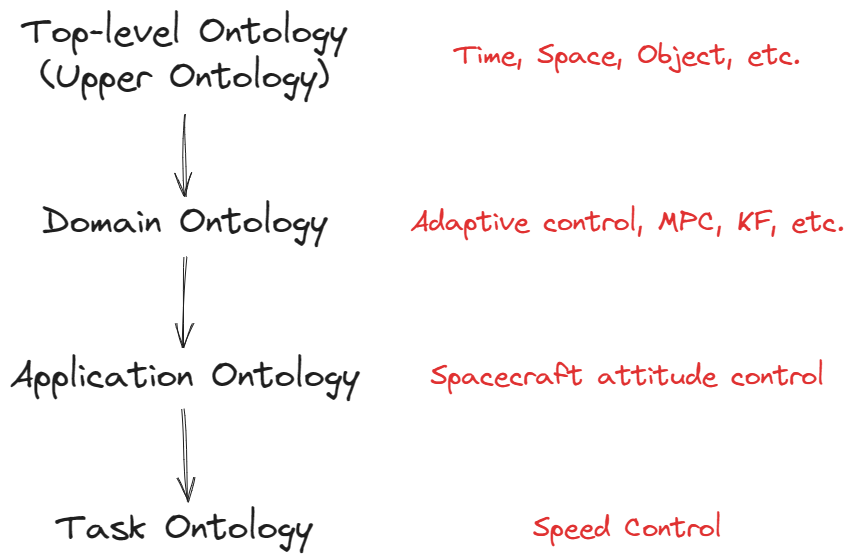
\includegraphics[width=0.6\textwidth]{chapters/part-4/figures/ontologylevel.png}
	\caption{A demonstrative example of ontology level using control engineering.}
	\label{fig:ontologylevel}
\end{figure}

Other ways of leveling ontology include using the expressiveness. The ``light-weight'' ontology is informal, less semantic, and supports less comprehensive logic. The ``heavy-weight'' ontology, on the other hand, is formal, more semantic, and supports more comprehensive logic and reasoning up to first-order logic. The vocabulary also grows with the ontology complexity.

\section{Logic} \label{sec:logic}

Humans are good at deriving new knowledge from existing knowledge. The systematic way of doing so is \mync{logic}. The term ``formal logic'' rigorously defines logic reasoning methods and procedures to automate logic inference by machines.

Notice that logic and logical expression are by themselves very complex and rich concepts. It is not possible to include all the details about them in the scope of this notebook. Only a brief scratch is given.

\subsection{Different Semantics from the Same Syntax}

Given the same information, different people and/or machines can draw different semantics. Consider the following example. This is a piece of code written in Python.
\begin{lstlisting}
ax = []
for i in range(20):
	if i<=1:
		ax.append(i)
	else:
		ax.append(ax[i-1]+ax[i-2])
\end{lstlisting}
Three interpreters are studied, the Python interpreter, the AI model, and the human cognition. Different interpreters draw different semantics from the same code above.

The Python interpreter is purely syntax-driven. When it executes a script, it follows the provided instructions without any broader comprehension or anticipation of what the code is doing. In the context of this example, the interpreter does not recognize that it is generating the famous Fibonacci sequence. It simply follows the rules of the script, calculating and outputting each number in the series as instructed.

On the other hand, an AI model like GPT-3 does possess a level of semantic understanding. Through training on massive data corpus especially codes, it can associate the above Python script with Fibonacci series. This understanding is not innate but rather a result of statistical inference and pattern matching from the training data. In other words, in the training data there are similar codes which is referred as ``the code to generate Fibonacci series''. When asked about the script, it can provide a summary or explanation based on its learned associations, including the name of the series and the purpose of each line of the code. It can even suggest improvement or fix bugs, so long as in the training data a more efficient realization of the code is provided.

Finally, there's the human level of semantics, which is by far most advanced and intuitive. Not only can a human understand the Python script and the concept of the Fibonacci series, they can also infer its broader mathematical properties, such as its relation to the golden ratio, and its general behavior. One good at mathematics can intuitively understand that the series will converge to the golden ratio not only when starting with 0 and 1 but with any two initial positive integers, even if he is not specifically taught that knowledge. This level of understanding is a combination of learned knowledge, pattern recognition, and the ability to extrapolate or generalize from existing information.

One of the goals of semantic web is to enable a machine to understand the semantics as much as possible, hopefully to gain the capability of logic reasoning just like a human. 

\subsection{Logic Framework} \label{subsec:knowledgeandlogic}

Different logic frameworks have different levels of complexity, hence different capabilities of expressing semantics. Commonly seen logic frameworks are briefly introduced as follows.

\vspace{0.1in}
\noindent \textbf{Propositional Logic}
\vspace{0.1in}

Propositional logic is the fundamental of logic reasoning. In propositional logic, knowledge is represented by either simple facts which are known as propositions, or facts connected with ``AND'', ``OR'', ``NOT'', ``IF ... THEN ...'', ``IF AND ONLY IF'' which are known as compound propositions.

\vspace{0.1in}
\noindent \textbf{First-Order Logic}
\vspace{0.1in}

\myabb{First-order logic}{FOL} is the most commonly used logic as of today. In FOL, quantifiers and logic connectives are introduced, including universal quantification $\forall$, existential quantification $\exists$, conjunction $\land$, disjunction $\lor$ and negation $\neg$. A formal way of representing logic expressions are defined. For example, using the following to represent ``all humans are mortal''
\begin{eqnarray}
	\forall x \left(\textup{Human}(x) \rightarrow \textup{Mortal}(x)\right) \nonumber
\end{eqnarray}
where $\textup{CLASS}(x)$ is equivalent of a proposition ``$x$ belongs to CLASS'', which can be either true or false. The above proposition says ``for any item, if it is true that the item belongs to human, then it must be true that the item belongs to mortal''.

\vspace{0.1in}
\noindent \textbf{Description Logic}
\vspace{0.1in}

\myabb{Description logic}{DL} is a subset of FOL. Derivation of DL from FOL is not under the scope of this notebook. Some key features of DL are summarized as follows.
\begin{itemize}
	\item Define classes and subclasses.
	\item Define properties (roles) and associated domains and ranges.
	\item Define restrictions on classes and properties.
	\item Support universal and existential quantifiers.
\end{itemize}
Semantic web uses OWL to implement DL on computers. More details are given in Section \ref{sec:owl}.

\begin{shortbox}
	
\Boxhead{Undecidability in FOL}

We would surely want to introduce highly expressive and complex formalisms to the existing RDF/RDFS model. This motivates OWL, which enables DL in semantic web. More details of OWL is introduced later in Section \ref{sec:owl}. 

Notice that DL instead of FOL is widely used in semantic web due to the fact that FOL is undecidable.

A logic is decidable if there is an algorithm that can determine whether any given statement in the logic is true or false. If no such algorithm exists for a logic, it is undecidable. G$\ddot{o}$del's Incompleteness Theorems indicates that in any sufficiently powerful logical system such as FOL, there are statements that are true but cannot be proven within the system. FOL, therefore, is undecidable. An FOL reasoning algorithm may not terminate in finite time. The proof of this theorem can be found elsewhere and is not given in this notebook.

While FOL inference is not decidable, DL inference, on the other hand, is decidable. That is one of the reasons DL is preferred over FOL in semantic web.
	
\end{shortbox}

\mync{Attributive language with complement}[ALC] is one of the ways to describe a simple DL, and it forms an important subset of OWL. Understanding ALC is helpful with learning OWL in later sections. A brief introduction of ALC is given below.

``Concept'' (corresponding with class in RDF/RDFS) and ``role'' (corresponding with property in RDF/RDFS) are introduced in ALC. Top concept (root class) and bottom concepts (leaf classes) are defined. Each property is associated with a range, which is basically a set of values that the property can take.

Constructors are used to describe the concepts, roles and ranges used in ALC. Conjunction, disjunction, negation, existential and universal quantifiers are supported. For example, let $R$ be a role and $C$ be a concept, and $\forall R.C$ means that all roles ``$R$'' must take values from concept ``$C$''. Likewise, $\exists R.C$ means that there is at least one role ``$R$'' whose value is taken from concept ``$C$''. Concept relations are defined. Commonly used concept relation constructors are inclusion (to describe subclass), equality (to assign class), union, intersection, complement, etc.

ALC uses \mync{terminological knowledge statements} (define concepts and roles schema) and \mync{assertional logic statements} (insert instances) to record knowledge. Examples are given below. Using terminological knowledge we can define a teacher as
\begin{lstlisting}[mathescape=true]
Teacher $\equiv$ Person $\land$ $\exists$ HasStudent.Student $\land$ $\exists$ Teaches.Lecture
\end{lstlisting}
which translates to ``a Teacher is a Person, and it has at least one role HasStudent whose value is from Student, and has at lease one role Teaches whose value is from Lecture'', where ``Person'', ``Student'', ``Lecture'' are concepts and ``HasStudent'', ``Teaches'' are roles. There are also teachers who teach only tutorials but not classes. To include them into the Teacher class, consider using
\begin{lstlisting}[mathescape=true]
Teacher $\equiv$ Person $\land$ $\exists$ HasStudent.Student $\land$ ($\exists$ Teaches.Lecture $\lor$ $\exists$ Teaches.Tutorial)
\end{lstlisting}
With terminological knowledge, ALC can enforce restrictions on concepts and rules flexibly. Using assertional knowledge, on the other hand, allows defining instances and subclasses as follows.
\begin{lstlisting}
Teacher(Peter)
Lecture(Calculus)
Teaches(Peter, Calculus)
\end{lstlisting}

All the above ALC can be translated into OWL then implemented in the semantic web. More details are given in later sections.

\subsection{Logical Expression}

A logic is defined by 
\begin{eqnarray}
	L&:=& (S, \models) \nonumber
\end{eqnarray}
where $S$ is the set that contains all the statements of our interests, and $\models$ the entailment relation
\begin{eqnarray}
	\models &=& \models^1 \bigcup \models^2 \nonumber
\end{eqnarray}
where
\begin{eqnarray}
	\models^1 &=& \left\{(\Phi,\phi)\middle| \Phi \subseteq S, \phi\in S, \Phi\rightarrow \phi\right\} \label{eq:logicentailment} \\
	\models^2 &=& \left\{(\Phi, \Psi)\middle| \Phi, \Psi \subseteq S, \forall \psi \in \Psi, \Phi \models^1 \psi \right\} \label{eq:compoundlogicentailment}
\end{eqnarray}

In \eqref{eq:logicentailment}, $\phi$ is known as the logical consequence of $\Phi$. If two logical assertions satisfy $\Phi \models \Psi$ and $\Psi \models \Phi$, then they are logically equivalent $\Phi \equiv \Psi$.

A logic statement is meaningful only if its interpretation $I$ and formula $F$ are clearly articulated. $I$ and $F$ are two very important terms in logic expression. \mync{Logic interpretation} is a formal construct that defines the meaning of a symbol in a formal language. For example, in the ontology of people, an interpretation can map an instance symbol, such as ``Alice'', to an actual person in the real world, and class symbol ``Person'', to the concept of a human being, etc. \mync{Logic formula}, on the other hand, is a statement formulated by string of symbols from a formal language. It is an assertion trying to represent some fact. For example, a formula can be ``Alice hasSibling Bob''. 

The true or false of the formula depend not only by the formula itself, but also by the interpretation. In the earlier example ``Alice hasSibling Bob'', if ``Alice'' and ``Bob'' are indeed mapped to two siblings, and the relation ``hasSibling'' is as it literally represents, then it is true. Here is another example. Consider formula ``10 is greater than 5''. Intuitively, this is a universal truth. But from the interpretation and formula perspective, this also depends on the interpretation. If ``10'' and ``5'' are interpreted as numerical quantities and ``is greater than'' as the standard numerical greater-than relation, then it is true. However, if ``10'' and ``5'' are interpreted as amounts of debt and ``is greater than'' as ``richer'' (with less debt being richer), then it would be false under this interpretation.

The interpretations that make the formula true form the model of the formula denoted by $I(F)$ or $I \models F$, which read as ``I models F'' or ``I satisfies F''. 

With the above, we can express FOL using logic expression. Here is an example
\begin{eqnarray}
	\forall X: \textup{Child}(X) \rightarrow \textup{lovesIcecream}(X) \nonumber
\end{eqnarray}
which says ``for all elements denoted by $X$, if $X$ interpreted as Child holds true, then $X$ interpreted as lovesIcrcream must also be true''.

Multiple formulas can be grouped into a theory ($T$), which can be used interchangeably with F. A theory can be treated as a knowledge base.

\subsection{Logical Equivalence}

Logical equivalence has already been introduced earlier. Recall \eqref{eq:compoundlogicentailment} where we say if $\Phi \models \Psi$ and $\Psi \models \Phi$, $\Phi$ and $\Psi$ are logically equivalent denoted by $\Phi \equiv \Psi$. Here $\Phi$ and $\Psi$ are sets of statements.

Consider a simplified case where $\Phi$ and $\Psi$ each contains only one statement. Let the formula of the statements of $\Phi$ and $\Psi$ be $F$ and $G$ respectively. The notations applied to $\Phi$ and $\Psi$ applies to $F$ and $G$ similarly. For example, $F\models G$ means that under the same interpretation if $F$ is true, $G$ must also be true. If $F \models G$ and $G \models F$, $F$ and $G$ are logically equivalent denoted by $F\equiv G$.

There is a huge table of logical equivalence formulas. Commonly seen equivalence is given in Table \ref{tab:logicalequivalence}. The proof of the formulas is not given here. The interpretation of conjunction $\land$, disjunction $\lor$ and negation $\neg$ are ``AND'', ``OR'', ``NOT'' respectively.
\begin{table}
	\centering \caption{Numerical calculations.} \label{tab:logicalequivalence}
	\begin{tabularx}{\textwidth}{llX}
		\hline
		Statement & Equivalent & Comment \\
		\hline
		$\neg \neg p$ & $p$ & Double negation law \\
		$(p \land q)$ & $(q \land p)$ & Commutative law \\
		$(p \lor q)$ & $(q \lor p)$ & Commutative law \\
		$(p \land (q \land r))$ & $((p \land q) \land r)$ & Association law \\
		$(p \lor (q \lor r))$ & $((p \lor q) \lor r)$ & Association law \\
		$(p \land (q \lor r))$ & $((p \land q) \lor (p \land r))$ & Distributive law \\
		$(p \lor (q \land r))$ & $((p \lor q) \land (p \lor r))$ & Distributive law \\
		$(p \rightarrow q)$ & $(\neg p \lor q)$ & Conditional statements \\
		$(p \rightarrow q)$ & $(\neg q \rightarrow \neg p)$ & Conditional statement \\
		$(p \leftrightarrow q)$ & $((p \rightarrow q) \land (q \rightarrow p))$ & Conditional statement \\
		$(\neg (p \land q))$ & $(\neg p \lor \neg q)$ & De Morgan's law \\
		$(\neg (p \lor q))$ & $(\neg p \land \neg q)$ & De Morgan's law \\
		\hline
	\end{tabularx}
\end{table}

Canonical forms have been defined for logical expressions. There are at least 6 different canonical forms for a logical expression, namely conjunctive normal form, disjunctive normal form, prenex normal form, skolem normal form, negation normal form and clausal normal form. Canonical forms are not necessarily the easiest and most intuitive forms of an expression (in fact it is quite the opposite), but somethings they are simple for further analysis and process, such as finding contradictions.

Notice that when deriving certain canonical forms from the original logical expression, information may get lost and they are not necessarily always equivalent, but they usually are.

\subsection{Logical Reasoning}

Logical reasoning is about proving true or false of a formula $F$ given a theory $T$. The proof may not be unique, and sometimes it is difficult to find one.

Before talking about how knowledge is retrieved from the knowledge base using DL inference and reasoning, we need to discuss what to return if knowledge is not found. When open world assumption (OWA) is made, the knowledge base considers itself as underdevelopment, and it is open-minded to unknowns. While when closed world assumption (CWA) is made, the knowledge base considers itself as developed, and unknown means nonexistence.

Consider an example where it is asked ``are Alice's children all males?'', and in the database there are two children of Alice, both of which are male. Under OWA, the inference would return ``maybe'', as it does now know whether there are more children of Alice. While in CWA, the inference would return ``yes'', as it checks both children to be male, and it assumes they would be all the children Alice has. However, when Alice does have female child registered, both OWA and CWA inferences would return ``no'', because the female child contradicts the assertion regardless of the completeness of the database.

The law of contradiction is widely used in logic reasoning. For example, to prove $T\models F$, just find contradictions in $\{\neg F, T\}$. A commonly used way of looking for contradictions in $\{\neg F, T\}$ is to resolve the formula into something more structured, for example to one of its canonical forms. Commonly used canonical forms for contradiction check are clausal normal form and disjunctive normal form.















